%%%%%%%%%%%%%%%%%%%%%%%%%%%%%%%%%%%%%%%%%%%%%%%%%%%%%%%%%%%%%%%%%%%%%%%%%%%%%%%%
%2345678901234567890123456789012345678901234567890123456789012345678901234567890
%        1         2         3         4         5         6         7         8

\documentclass[letterpaper, 10 pt, conference]{ieeeconf}  % Comment this line out if you need a4paper

%\documentclass[a4paper, 10pt, conference]{ieeeconf}      % Use this line for a4 paper

\IEEEoverridecommandlockouts                              % This command is only needed if 
                                                          % you want to use the \thanks command

\overrideIEEEmargins                                      % Needed to meet printer requirements.

% See the \addtolength command later in the file to balance the column lengths
% on the last page of the document

% The following packages can be found on http:\\www.ctan.org
\usepackage{graphics} % for pdf, bitmapped graphics files
\usepackage{graphicx}
%\usepackage{epsfig} % for postscript graphics files
%\usepackage{mathptmx} % assumes new font selection scheme installed
%\usepackage{times} % assumes new font selection scheme installed
\usepackage{amsmath} % assumes amsmath package installed
%\usepackage{amssymb}  % assumes amsmath package installed
\newcommand\numberthis{\addtocounter{equation}{1}\tag{\theequation}}
\graphicspath{ {images/} }

\title{\LARGE \bf
Raag detection using Hidden Markov Models
}


\author{Dhruva Kumar}% <-this % stops a space

\begin{document}



\maketitle
\thispagestyle{empty}
\pagestyle{empty}


%%%%%%%%%%%%%%%%%%%%%%%%%%%%%%%%%%%%%%%%%%%%%%%%%%%%%%%%%%%%%%%%%%%%%%%%%%%%%%%%
\begin{abstract}

The task of \textit{raag} detection is attempted using Hidden Markov Models (HMM). Every \textit{raag} is characterized uniquely by certain melodic transitions. HMM is used to learn these unique transitional probablities for every \textit{raag}. By using only the pitch contour as a feature, HMM works quite well by identifying a test set of 16 samples spanning across different modalities with an accuracy of 81.25\%.

\end{abstract}


%%%%%%%%%%%%%%%%%%%%%%%%%%%%%%%%%%%%%%%%%%%%%%%%%%%%%%%%%%%%%%%%%%%%%%%%%%%%%%%%
\section{INTRODUCTION}

A \textit{raag} is a melodic concept in Indian Classical Music (ICM) on which most of the songs from the ICM domain are based on. Technically, a \textit{raag} is a combination of a set of melodic notes played or sung in a specific way. The melodic notes and the transition between these notes are defined for every \textit{raag} and uniquely characterize them. These chararcteristic sequences are called \textit{aaroh} (ascending sequence), \textit{avroh} (descending sequence) and \textit{pakad} (a succinct sequence which contains both the ascent and descent). Based on top of these technical rules for the given \textit{raag}, a \textit{raag} performance consists of various ornamental embellishments and nuances like \textit{meend} (glissando), \textit{kan-swar} (grace notes) and \textit{gamaks} (a percussive voice production technique) which are used to bring out the essence and flavor of the \textit{raag}. Every \textit{raag} performance is associated with a \textit{rasa} or an emotion which is brought out vividly through these nuances. 
Certain notes are held longer and are emphasized more than the others. These are called \textit{vadi} (most important) \textit{swar} (note). The second most important note is called the \textit{samvadi swar}. \\
The melodic notes of a \textit{raag} are based on the chromatic scale and a \textit{raag} generally consists of 5 to 12 chromatic pitches. Most of the \textit{raag} performances are based on the three octaves C3 to B5 (\textit{mandra}, \textit{madhya} and \textit{taar} \textit{saptak}) and this range is considered for the quantization of pitch features. \\
Every \textit{raag} performance has a drone tone (\textit{tanpura}) played continuously in the background. The pitch of this drone tone is the tonic frequency set by the musician for the recording. \\

The present work uses Hidden Markov Models in an attempt to learn the transitional probabilites between the melodic notes which uniquely defines a \textit{raag} as described previously. 


%%%%%%%%%%%%%%%%%%%%%%%%%%%%%%%%%%%%%%%%%%%%%%%%%%%%%%%%%%%%%%%%%%%%%%%%%%%%%%%%
\section{MOTIVATION}

Identifying a \textit{raag} is important for musicians in finding the underlying key for every musical piece. The task of identifying a \textit{raag} is currently done by trained classical musicians with 10 to 15 years of experience. \\
Identifying a \textit{raag} is also useful for musical therapy. By understanding which type of \textit{raag} the person likes to listen to and therefore the emotions or \textit{rasa} associated with it, one can get an insight into the person's psychological experience. \\
It can also be used in music recommendation systems where similar songs can be generated in the playlist. Here, the similarity index is the underlying \textit{raag} or the underlying mood of the person at the time. 

%%%%%%%%%%%%%%%%%%%%%%%%%%%%%%%%%%%%%%%%%%%%%%%%%%%%%%%%%%%%%%%%%%%%%%%%%%%%%%%%
\section{RELATED WORK}

Automatic \textit{raag} classification has been discussed and attempted previously. Various methods have been used like pitch class distribution (PCD), HMM, finite automata modeling of the musical rules, pitch class string formation.  \\
\cite{c3} uses PCDs and pitch-class dyad distributions (PCDDs) as features derived from pitch contours. PCDDs are essentially bi-grams of pitch classes. The pitch contour was detected  using the Harmonic Product Spectrum (HPS) algorithm. The dimensionality of the features was reduced to 50 from 156 using PCA and a Multivarite Normal (MVN) classifier was applied. An accuracy of 94\% was was achieved on a test set of 17 samples. 17 \textit{raag} classes were used. GTraagDB \cite{c2} was used as the dataset. \\
\cite{c4} uses HMM and a string matching algorithm to detect \textit{raags}. The pitch contour was used as the feature which was detected using the autocorrelation metod. Only 2 \textit{raag} classes were used and an accuracy of 77\% was achieved on test set of 31 samples. An improved performance of 10\% was achieved with an additional stage that involved identifying catch phrases called \textit{pakad} in the test sequences. The dataset used was collected manually.  

%%%%%%%%%%%%%%%%%%%%%%%%%%%%%%%%%%%%%%%%%%%%%%%%%%%%%%%%%%%%%%%%%%%%%%%%%%%%%%%%
\section{METHOD}

\subsection{Dataset}
A subset of GTraagDB \cite{c2} was used for training and testing. GTraagDB consists of 31 raags of duration ranging from 3 minutes to 60 minutes. The recordings consists of solo vocals and solo instruments. The percussions and the drone typically heard in \textit{raag} performances have been removed from the recordings. Each raag is also annotated with its tonic frequency.

\begin{table}[h]
\centering
\caption{\textit{Raag} classes used for training and its pitches}
\label{raag_class}
\begin{tabular}{ll}
\textit{\textbf{Raag}} & \textbf{Pitches used in the raag} \\
Bihag                  & C D E F F\# G A B                 \\
Darbari                & C D Eb F G Ab Bb                  \\
Desh                   & C D E F G A Bb B                  \\
Gaud Malhar            & C D E F G A Bb B                  \\
Yaman                  & C D E F F\# G A B                 
\end{tabular}
\end{table}

   \begin{figure}[thpb]
      \centering
      \framebox{\parbox{3in}{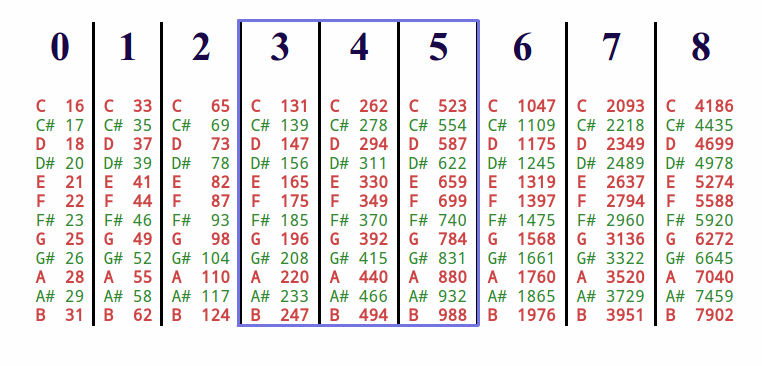
\includegraphics[width=3in]{1_octaves}}}
     % 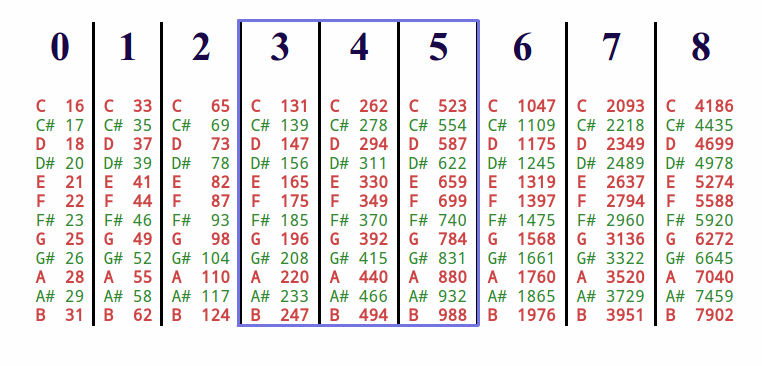
\includegraphics[width=3.5in]{1_octaves}
      \caption{Range of pitch scales chosen for pitch quantization as shown by the blue bounding box. Includes the middle three octaves, \textit{mandra} (C3-B3), \textit{madhya} (C4-B4) and \textit{taar} (C5-B5) \textit{saptak}}
      \label{figurelabel}
   \end{figure}
   
Since enough samples were not present for each raag class, only 5 raag classes were used for training. 
% insert table 1 for these raag classes and the melodic notes used
Each raag class in the training set consist of 3 recordings of the sarod and sitar. The test set consists of 16 samples of vocals and sitar.

   
\subsection{Feature extraction, quantization and normalization}
A pitch contour for the input recording was obtained using Praat \cite{c2}. Praat uses an enhanced autocorrelation function to estimate the most likely pitch for every window of the waveform. Post processing is done to choose the most likely pitch path across the windows. This is done to prevent octave errors. 
   
Other popular methods for pitch detection like Yin \cite{c3} were tested for various samples in the dataset, but Praat gave the best results for most of them. 

The continous pitch contour for all the recordings were then quantized to the nearest chromatic scale pitch frequency. The relation between the frequency and the chromatic scale pitch for a 88 key piano is given by the following formula:

\begin{align*}
	f(n) =&\;  \sqrt[12]{2}^{(n-49)} \times 440 Hz \numberthis
\end{align*}

where n is the key number on the piano. The 49th key on a 88 key piano is A4 and it has a frequency of 440 Hz. 
Since each recording is performed in a different scale, there is a need for normalization to shift the recordings to a standard scale. This is done by the annotated tonic frequency for each recording in the dataset.
The quantized pitch above is normalized relative to C4 which has a frequency of 261.63 Hz. 
Only the middle three octaves, C3 to B5, are considered for pitch quantization since most of the raag performances are within this range. In the Indian Classical Music domain, these are called the \textit{mandra}, \textit{madhya} and \textit{taar} \textit{saptak}. This leads to a total of 36 quantization levels. 


\subsection{Learning: Baum Welch }
The HMM model was learnt using the Baum Welch procedure. It is an iterative EM procedure alternating between the E and M step, trying to maximize the cost function $P(O|\lambda)$ until the convergence criteria is met. \\

\paragraph{Initialization}
The HMM model was initialized to a fully connected structure. The initial state vector $\pi$ was uniformly distributed. The probability of starting from any state was equal. The transition matrix, $A$ and the emission matrix $B$ were randomly initialized. The number of hidden states $N$ was chosen to be 36. The idea was that at any given time, the pitch can lie in any of the chosen chromatic scale pitch state. The number of discrete observations $M$ was determined by the 36 quantization levels as described in the previous section. \\

\paragraph{Expectation}
The expectation step consists of computing the probability of the observation sequence given the model $P(O|\lambda)$. This is done by calculating the forward and backward variables $\alpha$ and $\beta$. The scaling used was as described in \cite{c1}.

\begin{itemize} 
\item Forward procedure:
\begin{enumerate}
	\item Initialization:
	\begin{align*}
	\alpha_1(i) =&\; \pi_i b_i(O_1) & 1 \leq i \leq N \\
	c_1 =&\; \frac{1}{\sum_{i=1}^N \alpha_1(i)}  \\
	\hat{\alpha_1}(i) =&\; c_1 \alpha_1(i) 
	\end{align*}
	
	\item Induction:
	\begin{align*}
	\alpha_{t+1}(j) =&\; [ \sum_{i=1}^N \alpha_t(i) a_{ij} ] \ b_j(O_{t+1})\numberthis  \\
	&\; 1 \leq t \leq T-1, \ 1\leq j \leq N \\
	c_t =&\; \frac{1}{\sum_{i=1}^N \alpha_t(i)} \numberthis \\
	\hat{\alpha_t}(i) =&\; c_t \alpha_t(i) \numberthis
	\end{align*}

	\item Termination:
	\begin{align*}
	P(O|\lambda) =&\; \sum_{i=1}^N \alpha_T(i)  \\
	=&\; \frac{1}{\prod_{\tau=1}^T c_{\tau}} \\ 
	\log{P(O|\lambda)} =&\;  -\sum_{t=1}^T \log{c_t}  \numberthis \\
	\end{align*}
\end{enumerate}
Equation (4) gives the value of the forward variable after scaling.

\item Backward procedure:
\begin{enumerate}
	\item Initialization:
	\begin{align*}
	\beta_T(i) =&\; 1  & 1 \leq i \leq N \numberthis \\
	\hat{\beta_T}(i) =&\; c_T \beta_T(i)
	\end{align*}

	\item Induction:
	\begin{align*}
	\beta_T(i) =&\; \sum_{j=1}^N a_{ij} b_j(O_{t+1}) \beta_{t+1}(j) \\
	&\; T-1 \geq t \geq 1, \ 1 \leq i \leq N \\
	\hat{\beta_t}(i) =&\; c_t \beta_t(i)	
	\end{align*}

\end{enumerate}
The scaling in (3) is used here.
\end{itemize} 
For multiple sequences, $\alpha^l$, $\beta^l$ and $c^l$ is computed for each sequence $l$. \\

\paragraph{Modification}
Given the forward and backward variables, the model parameters ${\pi, A, B}$ are updated so that the cost function $P(O|\lambda)$ is maximized. The re-estimated paramters {$\overline{\pi}$, $\overline{A}$, $\overline{B}$} are as follows:

\begin{align*}
	\overline{\pi_i} =&\; \text{expected number of times in state}\\
					&\; S_i \text{ at time } (t = 1)  \\
	=&\; \gamma_1(i) \\ \\
	\overline{a}_{ij} =&\; \frac{\text{expected number of transitions from state }S_i \text{ to } S_j}{\text{expected number of transitions from state }S_i} \\
	=&\; \frac{\sum_{t=1}^{T-1} \xi_t(i,j)}{\sum_{t=1}^{T=1}\gamma_t(i)} \\
	=&\; \frac{\sum_{t=1}^{T-1} \alpha_t(i) a_{ij} b_{j}(O_{t+1}) \beta_{t+1}(j)}{\sum_{t=1}^{T-1} \alpha_t(i) \beta_{t}(j) } \\
	=&\; \frac{\sum_{t=1}^{T-1} \hat{\alpha}_t(i) a_{ij} b_{j}(O_{t+1}) \hat{\beta}_{t+1}(j)}{\sum_{t=1}^{T-1} \hat{\alpha}_t(i) \hat{\beta}_{t}(j) / c_t } \\ \\
	&\; \text{For multiple observations, }\\
	=&\; \frac{\sum_{l=1}^{L-1} \sum_{t=1}^{T_l-1} \hat{\alpha}_t^{l}(i) a_{ij} b_{j}(O_{t+1}^{l}) \hat{\beta}_{t+1}^{l}(j)}{\sum_{t=1}^{T_l-1} \hat{\alpha}_t^{l}(i) \hat{\beta}_{t}^{l}(j) / c_t^{l} } \numberthis \\ \\
	\overline{b}_j(k) =&\; \frac{\text{expected no. of times in state } j \text{ with symbol }\upsilon_k}{\text{expected no. of times in state }j} \\
	=&\; \frac{\sum_{t=1, O_t=\upsilon_k}^{T} \gamma_t(j)}{\sum_{t=1}^{T} \gamma_t(j)} \\
	=&\; \frac{\sum_{t=1, O_t=\upsilon_k}^{T} \hat{\alpha}_t(j) \hat{\beta}_t(j) / c_t}{\sum_{t=1}^{T} \hat{\alpha}_t(j) \hat{\beta}_t(j) / c_t} \\ \\
	&\; \text{For multiple observations, } \\
	=&\;  \frac{\sum_{l=1}^{L} \sum_{t=1, O_t^{l}=\upsilon_k}^{T_l} \hat{\alpha}_t^{l}(j) \hat{\beta}_t^{l}(j) / c_t^{l}}{\sum_{t=1}^{T_l} \hat{\alpha}_t^{l}(j) \hat{\beta}_t^{l}(j) / c_t^{l}} \numberthis \\
\end{align*}


$\gamma_t(i)$ is the probability of being in state i at time t given the observations sequence and the model $\lambda$
\begin{align*}
	\gamma_t(i) =&\; P(q_t = S_i | O, \lambda) = \frac{\alpha_t(i) \beta_t(i)}{P(O | \lambda)} \numberthis \\ 
\end{align*}

$\xi_t(i,j)$ is the probability of being in state $S_i$ at time $t$ and $S_j$ at time $t+1$, given the model and observation sequence. 
\begin{align*}
	\xi_t(i,j) =&\; P(q_t = S_i, q_{t+1} = S_j | O,\lambda) \\
	=&\; \frac{\alpha_t(i) a_{ij} b_j(O_{t+1}) \beta_{t+1}(j)}{P(O|\lambda)} \numberthis \\
\end{align*}

\paragraph{Convergence criteria}
The EM steps were alternated iteratively until the convergence criteria was met. The convergence criteria was assigned as when the absolute of the difference in the log likelihood of $P(O|\lambda)$ between successive iterations was less than 0.1. \\

   \begin{figure}[thpb]
      \centering
      \framebox{\parbox{3in}{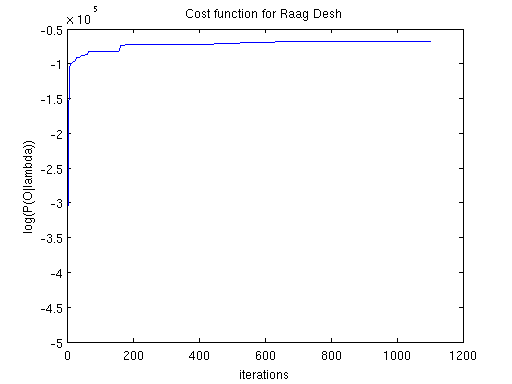
\includegraphics[width=3in]{2_costDesh}}}
     % 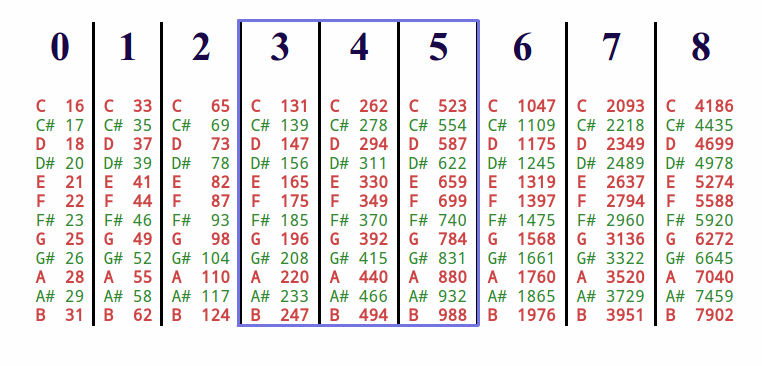
\includegraphics[width=3.5in]{1_octaves}
      \caption{The cost function: $\log P(O|\lambda)$ for \textit{raag desh} during training until the convergence criteria was met}
      \label{figurelabel}
   \end{figure}

%%%%%%%%%%%%%%%%%%%%%%%%%%%%%%%%%%%%%%%%%%%%%%%%%%%%%%%%%%%%%%%%%%%%%%%%%%%%%%%%
\section{Results}
Once the model parameters were learnt for each \textit{raag} class, each test sequence was tested using the forward-backward procedure as described before. The $argmax$ of $\log P(O|\lambda)$ among the \textit{raag} classes was chosen to be the detected \textit{raag} for the test sequence in subject.\\

An accuracy of 81.25\% was obtained on the test set. 13 out of 16 test samples were correctly identified. Out of the 16 test samples, 4 were solo vocal pieces and 12 were solo instrumentals. 11 out of 12 instrumental pieces were correctly identified. 2 out of 4 of the vocal pieces were correctly identified. The results are pretty good given the fact that vocal pieces were not included in the training data due to shortage of data. \textit{Raag desh} was misclassified twice as \textit{raag gaud malhar}. This can be explained by the fact that both the \textit{raags} share the same set of musical notes. They however differ in the transition between the notes. This transition was not accurately learnt by the HMM model. 

\begin{table}[h]
\caption{Confusion matrix on the test set}
\label{confusion}
\centering
\begin{tabular}{|c|c|c|c|c|c|}
\hline
            & Bihag & Darbari & Desh & Gaud M. & Yaman \\ \hline
Bihag       & 2     & 0       & 0    & 0       & 0     \\ \hline
Darbari     & 0     & 3       & 0    & 1       & 0     \\ \hline
Desh        & 0     & 0       & 1    & 2       & 0     \\ \hline
Gaud Malhar & 0     & 0       & 0    & 4       & 0     \\ \hline
Yaman       & 0     & 0       & 0    & 0       & 3     \\ \hline
\end{tabular}
\end{table}


This might be due to the pitch detection not always being correct. Another possibility is that the \textit{tanpura} drone which is played continuously in the background  in every piece might interfere with the notes that should be identified. A solution to this would be to identify and remove the drone tone in the preprocessing stage. 
All the test samples were accurately identified within the second or third best guess. 


   
%%%%%%%%%%%%%%%%%%%%%%%%%%%%%%%%%%%%%%%%%%%%%%%%%%%%%%%%%%%%%%%%%%%%%%%%%%%%%%%%
\section{Conclusion and future work}
Hidden Markov Model has proved to work quite well for \textit{raag} detection. It does a pretty good job of identifying the underlying transitional probabilites between the musical notes which is characteristic of every \textit{raag}. The current work was done on a small dataset. The next task would be to procure a strong training set in terms of quality so that the trained model would correctly identify test sequences spanning across different modalities. This can potentially be done by explicity adding the characteristic phrases, \textit{aaroh}, \textit{avroh}, \textit{pakad} and \textit{aalap} for every raag. The weights of these training sequences can be increased compared to the others so that the model learns the melodic tranisitions better. \\
As described previously, the sympathetic string drone sounds played in the background can be identified and removed during the preprocessing stage so that it doesn't interfere in the model learning the transitional probabilites. Another improvement is to use a better pitch detection algorithm. \\
   
   
In terms of features, more features like the amplitude can be incorporated in the training phase.  

   \begin{figure}[thpb]
      \centering
      \framebox{\parbox{3in}{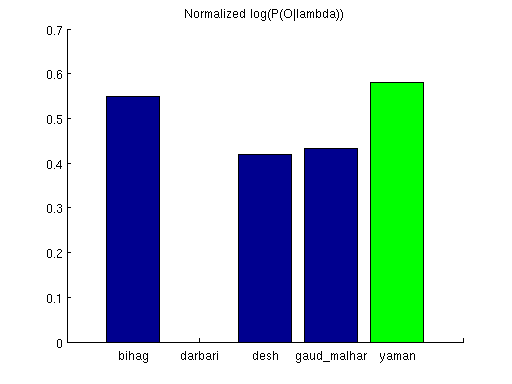
\includegraphics[width=3in]{3_log_p_1}}}
     % 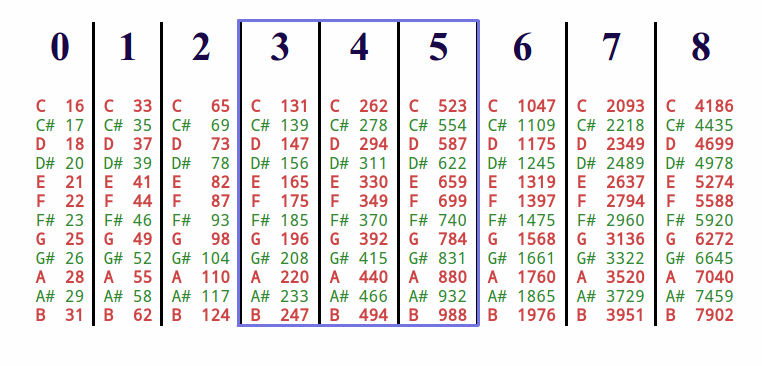
\includegraphics[width=3.5in]{1_octaves}
      \caption{The comparison of log likelihood of the test sequence (\textit{raag yaman}) given the models. Here, it correctly predicts the \textit{raag}. \textit{Raag bihag} comes close since it shares the same set of notes.}
      \label{figurelabel}
   \end{figure}
   
    \begin{figure}[thpb]
      \centering
      \framebox{\parbox{3in}{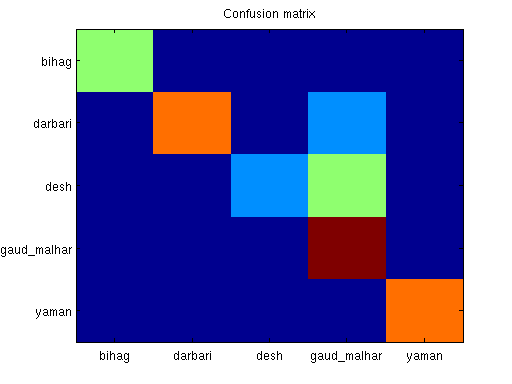
\includegraphics[width=3in]{conf}}}
     % 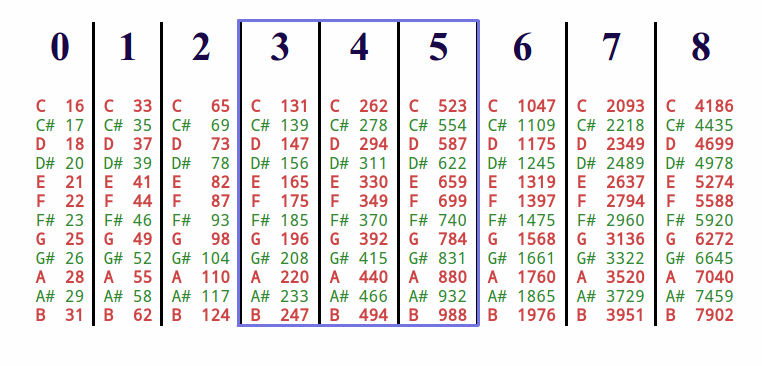
\includegraphics[width=3.5in]{1_octaves}
      \caption{Confusion matrix on the test set}
      \label{figurelabel}
   \end{figure}
   
         \begin{figure}[thpb]
      \centering
      \framebox{\parbox{3in}{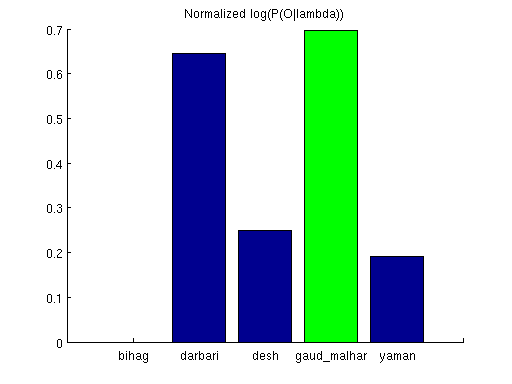
\includegraphics[width=3in]{4_log_p_2}}}
     % 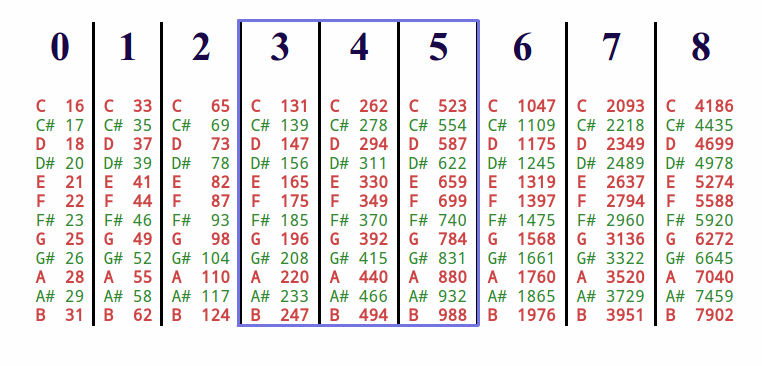
\includegraphics[width=3.5in]{1_octaves}
      \caption{\textit{Raag darbari} being misclassified as \textit{raag gaud malhar}}
      \label{figurelabel}
   \end{figure}
   
   
In addition to the unique sequences in every \textit{raag}, each \textit{raag} is also characterized by the most emphasized note, \textit{vadi} and the second most emphasized note \textit{samvadi}. This can be encoded as the amplitdue along with the pitch to be used as features. \\
In conclusion, HMM has proved to be quite a good candidate for \textit{raag} detection and there is scope for improvement to achieve better results. 


%%%%%%%%%%%%%%%%%%%%%%%%%%%%%%%%%%%%%%%%%%%%%%%%%%%%%%%%%%%%%%%%%%%%%%%%%%%%%%%%


\addtolength{\textheight}{-12cm}   % This command serves to balance the column lengths
                                  % on the last page of the document manually. It shortens
                                  % the textheight of the last page by a suitable amount.
                                  % This command does not take effect until the next page
                                  % so it should come on the page before the last. Make
                                  % sure that you do not shorten the textheight too much.

%%%%%%%%%%%%%%%%%%%%%%%%%%%%%%%%%%%%%%%%%%%%%%%%%%%%%%%%%%%%%%%%%%%%%%%%%%%%%%%%



%%%%%%%%%%%%%%%%%%%%%%%%%%%%%%%%%%%%%%%%%%%%%%%%%%%%%%%%%%%%%%%%%%%%%%%%%%%%%%%%



%%%%%%%%%%%%%%%%%%%%%%%%%%%%%%%%%%%%%%%%%%%%%%%%%%%%%%%%%%%%%%%%%%%%%%%%%%%%%%%%
%\section*{APPENDIX}
%
%Appendixes should appear before the acknowledgment.

\section*{ACKNOWLEDGMENT}

I would like to thank Dr. Dan Lee for the excellent lectures due to which understanding the content was a breeze. I would also like to thank Bhoram, Steve and Chris for their invaluable guidance.



%%%%%%%%%%%%%%%%%%%%%%%%%%%%%%%%%%%%%%%%%%%%%%%%%%%%%%%%%%%%%%%%%%%%%%%%%%%%%%%%


\begin{thebibliography}{99}

\bibitem{c1}  Lawrence R. Rabiner, "A Tutorial on Hidden Markov Models and Selected Applications in Speech Recognition": Proc. IEEE, Vol. 77, No. 2, pp. 257-286: February 1989.
\bibitem{c2} GTraagDB arranged by Parag Chordia, http://prernagupta.com/parag/data.html
\bibitem{c3} Chordia, P. 2006. "Automatic Raag Classification of Pitchtracked Performances Using Pitch-Class and Pitch-Class Dyad Distributions." In Proceedings of the International Computer Music Conference, pp. 314?321.
\bibitem{c4} Gaurav Pandey, et al "Tansen: A system for automatic Raga identification" IICAI, 2003 

\end{thebibliography}




\end{document}
